\chapter{Architecture}

In this section we will go through the architecture of HQL and describe how we
modelled the various of financial instruments in Haskell. We shall introduce
the necessary mathematical finance and conventions as we go along.

\section{Language features}

Functional languages lend themselves well to the domain of finance due
to several reasons such as modularity\cite{hughes:matters-cj}, 
laziness\cite{composingcontracts}[Section 5.3]. Moveover, the mathematical
 nature of finance makes functional languages suitable for valuation due its
inherent mathematical foundation and purity.\\

Haskell's advanced type system helps ensure that your code is safe, and its 
class system allows us to define type-safe interfaces for operations on 
financial products who themselves can be represented by Haskell data types. 
Statically typed languages have the advantage of discovering a multitude of
errors at compile time, and the type class system enables us to overload 
functionality in our programs based on our types. This is a very desirable
feature, as we want our financial products to have the same API (e.g. a function 
called \texttt{presentValue} should return the present value regardless of the
product type).

\section{Interest Rates}

We begin our introduction to mathematical finance with a concept familiar to
most, name interest rates. An interest rate is the the amount of return on
investing an amount of money for a set amount of time. This can be formulated
using a very simple equation, which we will demonstrate with a one year interest
rate on a deposits account:

\begin{equation}\label{eq:lincomp}
FV_T = N (1 + R_T)
\end{equation}

where $FV_T$ denotes the future value in $T$ time, $N$ is the nominal and $R_T$
is the rate over the period $T$\footnote{$T$ is also referred to as the
\emph{tenor}.}.) Extending this to multiple years (or periods) we introduce a new 
concept called compound interest, which is  simply the formula above reapplied
a number times. The intuitive approach is
that the compound interest is the return from reinvesting previously invested
capital. Mathematically, this return can be formulated as an exponentially 
compounded interest rate:

\begin{equation}\label{eq:expcomp}
FV_T^n = N (1 + R_T)^n
\end{equation}

where $FV$ is now dependent on the number of time it is compounded.
While this model is easy to understand, the world of finance demands much more 
intricate details to correctly understand it. Firstly, it assumes 
discrete time periods, but we have not specified if this $n$ stands for days, 
months, or years, or how what the tenor is. All of these intricacies are critical
for correctness of \hql and must be accounted for in the implementation.\\

Up until this point we have assumed that the compounding is performed at 
discrete intervals. However, as (1) is simply a formula, we may apply concepts 
from calculus to achieve what is known as the continuously compounded interest 
rate. It is defined as the resulting interest rate when we take the limit of 
equation \ref{eq:expcomp} as $n$ goes to infinity:

\begin{equation}
\text{lim}_{n \rightarrow \infty}\; FV_T^n \; = \; N (1 + R_T)^n
= N e^{RT}
\end{equation}

where $R$ is the continuously compounded interest rate.

The motivation behind the continuously compounded interest rate is that it is
much nicer to work with in more advanced fixed income modelling
\cite{cmunk}[Chapter 1] and yields almost identical numerical results.\\

\begin{figure}[!htb]
\centering
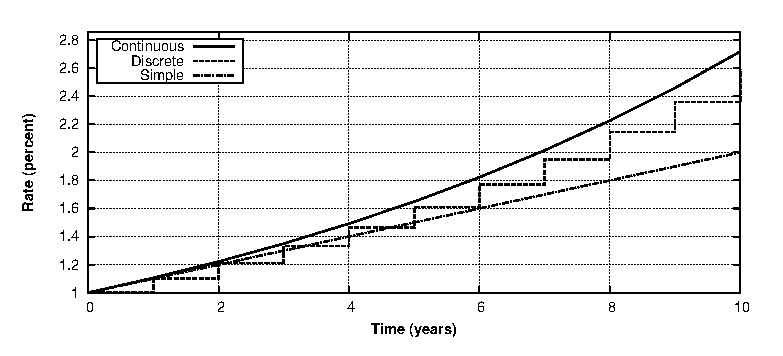
\includegraphics[scale=1.2]{images/comp02.eps}
\caption{How compounding methods influence returns.}
\label{fig:comp02}
\end{figure}

Figure \ref{fig:comp02} shows the influence in rate as a result of the different
kinds of compounding. Furthermore, table \ref{tab:cmptable} gives an overview of
the relation between compounding functions and time steps.It should be evident to 
the reader that the notion of linear continuously compounded interest rate is 
absurd, as we derive it from equation \ref{eq:expcomp}.

\begin{center}  
\begin{longtable}{|r|c|c|}
\hline  
\backslashbox{Time}{Compounding}
           &Linear  & Exponential\\\hline
Discrete   & Flat   & Periodic\\\hline
Continuous & \textcolor{red}{\xmark} & Continouous\\\hline
\caption{Compounding and time steps.}
\end{longtable}
\label{tab:cmptable}
\end{center}

We see that the method of compounding has very distinct impact on the returns.
From a modelling perspective, this means that we have designed Haskell
data types to distinguish between interest rates differing in the compound
method as follows:

\begin{hscode}
type Rate = Double
newtype ContinuousRate = ContinuousRate Rate deriving (Show)
newtype SimpleRate     = SimpleRate Rate deriving (Show) -- zero rate
data ExponentialRate   = ExponentialRate Rate Frequency deriving (Show)
\end{hscode}

Using the Haskell type system we can make sure that a continuously compounded
rate is not mistakenly used in a function that expects a zero rate.
Note that \texttt{newtype} does not exacerbate overhead.\\
Wishing to unify these different kinds of rates we have modelled an
\texttt{InterestRate} class that allows for abstraction of the underlying rate.

\begin{hscode}
type Offset         = Double -- yearly offset
type DiscountFactor = Double
class InterestRate r where
  -- | Returns the corresponding continuously compounded rate
  continuousRate :: r -> ContinuousRate
  -- | Returns the discount factor at an offset
  discountFactor :: r -> Offset -> DiscountFactor 
  -- | Reciprocal of the discount factor
  compoundFactor :: r -> Offset -> DiscountFactor 
  -- | Get the intrinsic rate
  rate           :: r -> Rate
\end{hscode}

It defines an interface for retrieval of rates regardless of the underlying
data type. As mentioned, advanced fixed income modelling and options pricing
often use the continuously compounded rates due to its mathematical 
properties\cite{HULL}. The \texttt{continuousRate} function caters to this
need, as it essentially solves the following equation for $R_C^n$:

\begin{equation}
e^{R_C^n} = (1+R_p)^n
\end{equation}.

where is $R_p$ the exponentially (periodically) compounded rate.\\

The \texttt{discountFactor} function introduces concept that we
explain in the following section.

We refer to the documentation\cite{hqldoc} for an in-depth treatment of the
mathematical finance pertaining to interest rates.

\section{Discounting}\label{sec:discounting}

We first present the basic theory of cashflow discounting, and motivate with
a small example. Given an option to invest an initial amount and receive DKK
$100$ in a year from now, how would you decide whether or not to invest? In
other words, what is the price of such an investment? If the investment bears
an interest rate of 5\%, then we may use equation \ref{eq:lincomp} to solve
for $N$:

\begin{equation}
100 = N (1 + 0.05) \Leftrightarrow N = \frac{100}{1+0.05}
\end{equation}

More generally, we have:

\begin{equation}
DF_T FV_T= N (1 + R_T)
\end{equation}

Meaning that our discount factor, $DF_T$, is $\frac{1}{1.05} \approx 95.238$
in the example above.\\

It is quite intuitive to think that the outcome of such a proposition depends 
on what alternatives are available. Assuming resources are limited, it may
quickly become difficult to asses which option is opportune if the market
offers multiple choices. This leads us onto the next key element in pricing
theory, namely the term structure of interest rates.\\

Again we refer the reader to the \hql documentation for more information.

\ab{This needs more work, but I hope you see where this is going.}

\section{Term Structure}

A term structure can be viewed as a function f that given a tenor returns 
an interest rate. Since these are zero rates, term structures are valuable 
tools in finance as we may use them to discount any cashflow regardless how it
was generated. The converse is not true, we cannot use the rate over the tenor
of a serial to discount a future income stream, unless that follows the exact
same cash flow pattern.\\

\begin{figure}[h!]
\begin{center}
\begin{tikzpicture}[-,shorten >=1pt,auto,node distance=1.5cm,thick,minimum size=0.8cm,main node/.style={circle,draw=red,very thick}]
\tikzstyle{selected edge} = [draw,line width=6pt,-,blue!30]
\coordinate (belowstart) at (0,-1);
\coordinate (xaxis) at (10,0);
\coordinate (origo) at (0,0);
\coordinate (yaxis) at (0,5);

% Draw axes
\draw[->] (origo) -- (xaxis) node[right] {Time to maturity};
\draw[->] (origo) -- (yaxis) node[above] {Interest rate};

% Flat TS
%\draw[thick,draw=blue] (0,1.5) -- (10,1.5);
% "Normal" TS
\draw[thick,draw=green] (0,0) parabola[bend at end] (10,5);
% Inverse TS
%\draw[thick,draw=red] (0,5) parabola[bend at end] (10,0.5);

\draw[dotted] (3,2.53) -- (3,0) node[below] {\text{ 3.5 years}};
\draw[dotted] (3,2.53) -- (0,2.53) node[left] {2.4\%};

% Legend
%\filldraw[draw=black, fill=blue] (5.2,-1) rectangle node {} +(0.2,0.2);
%\node at (6, -0.92) () {Flat};

%\filldraw[draw=black, fill=green] (0,-1) rectangle node {} +(0.2,0.2);
%\node at (1.55, -0.92) () {Logarithmic};

%\filldraw[draw=black, fill=red] (3,-1) rectangle node {} +(0.2,0.2);
%\node at (4.15, -0.92) () {Inverted};

\end{tikzpicture}
\caption{A example of a term structure.}
\label{fig:anc}
\end{center}
\end{figure}

A logarithmic shaped term structure as shown in \ref{fig:anc} characterizes a
"normal" market, where the return on an investment increases in some proportion
to the time you have tied up your funds\footnote{In reality, the shape depends on 
socio-economic factors such as growth or decline in the economy.}.\\

The term structure allows investors to observe at what price banks are
currently willing to loan money. We emphasize the time sensitivity of the term
structure, as external factors can cause sudden changes in the interest
rates and as a result the pricing of instruments (e.g. rate cuts by the
European Central Bank). By the time value of money it is possible to
appraise the value of an instrument (i.e. will the return on investment
be up to par with what a bank can offer?).\\

Turning to \hql, we need term structures to be able to price our instruments.
Like interest rates, term structures come in different flavours and we 
have therefore also defined a type class to represent them:

\begin{hscode}
class TermStructure a where
  -- | Returns the yield for a maturity
  yieldAt :: a -> Maturity -> Maybe Rate

  -- | Returns the discount factor at an offset
  dfAt :: a -> Maturity -> Maybe Rate
  dfAt a m = fmap recip $ yieldAt a m
 
  -- | Returns the discount factor at an offset
  fwdRate :: a -> Maturity -> Maturity -> Maybe DiscountFactor
  fwdRate a m0 m1 = (/) <$> dfAt a m1 <*> dfAt a m0
  
  -- | Returns the discount factors given a list of offsets
  dfsAt :: a -> [Maturity] -> [Maybe Rate]
  dfsAt a = map (dfAt a)
\end{hscode}

For instance, \texttt{yieldAt} function applied to the term structure in
figure \ref{fig:anc} with an offset of 3.5 years would produce $2.4\%$. We have
defined the following data types that are instances of the class above:

\begin{hscode}
newtype DiscreteTermStructure
  = DiscreteTermStructure (M.Map Maturity Rate)
newtype LinearInterpolatedTermStructure
  = LinearInterpolatedTermStructure (M.Map Maturity Rate)
newtype AnalyticalTermStructure
  = AnalyticalTermStructure (Offset -> Rate)
\end{hscode}

Moreover, the \texttt{TermStructure} class defines \texttt{fwdRate}, which
is a forward rate. There is no conceptual leap required to understand these,
as they are simply interest rates in the future, hence the type signature
requiring two offsets.

Notwithstanding, their usefulness is may not be evident. As mentioned, 
floating-rate bonds are defined by the fact that the interest rate is
non-deterministic. 

\ab{Explain forward rates!}
% TODO Talk about FWDRATES

\section{Fixed Income}

Now that we have cemented the basics of interest rates we will look at 
where they are applied, namely in which financial instruments. In this section
we will go through how we have modelled the subset of products called 
\emph{fixed income}, of which bonds are the bread and butter.\\
They are financial securities that promises the bond holder a
stream of future payments. These play a huge role in the financial markets are
are typically only offered by governments or large financial institutions.\\

We will present our \texttt{FixedIncome} module by means of a running example
of a bond. 
A \emph{serial} is an example of a bond that equates to a typical Danish house
loan. The cash flow of the holder of a 5 year serial with annual repayments is
depicted in figure \ref{fig:serialcf}.\\

\begin{figure}[h!]
\begin{center}
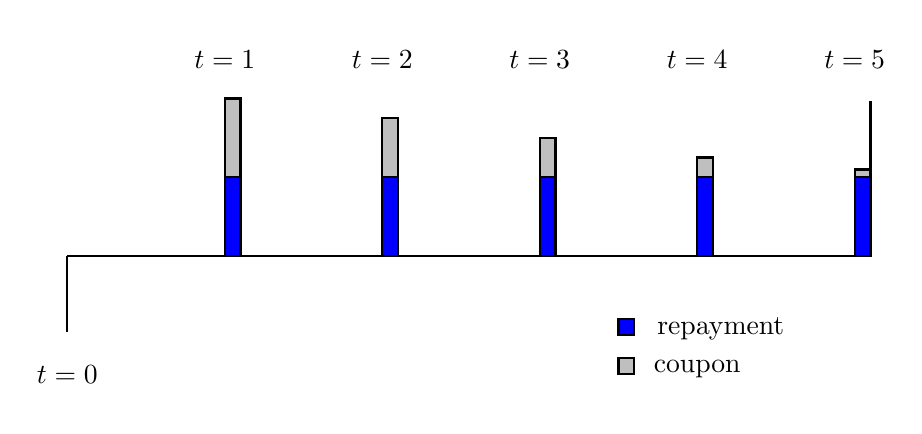
\begin{tikzpicture}[-,shorten >=1pt,auto,node distance=1.5cm,thick,minimum size=0.8cm,main node/.style={circle,draw=red,very thick}]
\tikzstyle{selected edge} = [draw,line width=6pt,-,blue!30]

\coordinate (belowstart) at (0,-1);
\coordinate (start) at (0,0);
\coordinate (stop) at (10.2,0);
\coordinate (abovestop) at (10.2,2);
\draw (start) -- (stop);
\draw (start) -- (belowstart);
\draw (stop) -- (abovestop);

\node at (0, -1.5) () {$t=0$};

\filldraw[draw=black, fill=blue] (2,0) rectangle node {} +(0.2,1);
\filldraw[draw=black, fill=lightgray]  (2,1) rectangle node {} +(0.2,1);
\node at (2, 2.5) () {$t=1$};

\filldraw[draw=black, fill=blue] (4,0) rectangle node {} +(0.2,1);
\filldraw[draw=black, fill=lightgray]  (4,1) rectangle node {} +(0.2,0.75);
\node at (4, 2.5) () {$t=2$};

\filldraw[draw=black, fill=blue] (6,0) rectangle node {} +(0.2,1);
\filldraw[draw=black, fill=lightgray]  (6,1) rectangle node {} +(0.2,0.5);
\node at (6, 2.5) () {$t=3$};

\filldraw[draw=black, fill=blue] (8,0) rectangle node {} +(0.2,1);
\filldraw[draw=black, fill=lightgray]  (8,1) rectangle node {} +(0.2,0.25);
\node at (8, 2.5) () {$t=4$};

\filldraw[draw=black, fill=blue] (10,0) rectangle node {} +(0.2,1);
\filldraw[draw=black, fill=lightgray]  (10,1) rectangle node {} +(0.2,0.1);
\node at (10, 2.5) () {$t=5$};

% Legend
\filldraw[draw=black, fill=blue] (7,-1) rectangle node {} +(0.2,0.2);
\node at (8.3, -0.92) () {repayment};

\filldraw[draw=black, fill=lightgray] (7,-1.5) rectangle node {} +(0.2,0.2);
\node at (8, -1.44) () {coupon};

\end{tikzpicture}
\caption{Cashflow of a serial.}
\label{fig:serialcf}
\end{center}
\end{figure}

We observe that the bond issuer makes fixed size deposits to the counterpart to 
repay the loan. Since there is no such thing as a free lunch, so-called coupon 
payments are made in addition to compensate for having its funds tied up. These
payments are simply the bond's interest rate applied to the face value of the
bond, and are decreasing as a result of the repayment amortization
\cite{hqldoc}.\\

In addition to the serial, we present the most basic bond imaginable, the zero 
coupon bond or simply \emph{zero}. It is exactly that - a bond with a specified 
tenor and interest rate that pays a fixed amount at maturity. As instruments and
bonds all come in multiple flavours we have designed a type class hiearchy to
model the complexity:

\begin{figure}[!htb]
\centering
%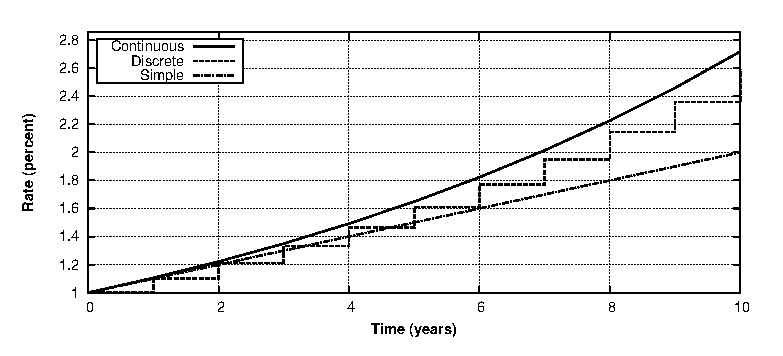
\includegraphics[scale=.7]{images/comp02.eps}
\texttt{images/tcarch.png}
\caption{Type class architecture.}
\label{fig:comp02}
\end{figure}

\ab{Delayed creating an image since I didn't 
think aethetics were critical for the draft.}

A central tenet of our architecture is that we keep the backend
as simple as possible and keep the interface detailed and 
self-explanatory. This way we keep the mathematical formulas as transparent
and clean as possible while the interface remains user-friendly.\\

\begin{center}
\texttt{<< Insert description of the class hierarchy and the awesomeness of
lists >>}\\
\end{center}

\ab{Discounting part needs to be intertwined with more Haskell goodness}.

Discounting in \hql can be seen as taking the dot product between the discount
factors and the cash flows at each point in time,

\[
p(0) = \mathbf{df}\cdot\mathbf{cf}
\]

Where the vector of discount factors, $\mathbf{df}$, and cash flow vector, $\mathbf{cf}$ are represented as

\[
\mathbf{df} = (p(t,T_1), ..., p(t,T_n)),
\]
\[
\mathbf{cf} = (c_1, ..., c_i).
\]

The fact that we model all bonds as list of zeros allows us to easily discount 
all bonds in the same manner. A functional programmer will already be thinking 
of this as a simple \texttt{map}, which is exactly how it is modelled in HQL.\\

For example, if we were to calculate the present value of a series of future cash flows,
	\[
	\mathbf{cf} = (\$1000.00,\$1500.00,\$1000.00,\$2000.00)
	\]
	We can multiply by the discount function with $T_n=n$ years and the rate at 5.00\% continuously compounded,
	\[
	p(0) = \mathbf{df}\cdot\mathbf{cf} = (e^{-rT_1},...,e^{-rT_n})\cdot(p(0,T_1), ...,p(0,T_4))=
	\]
	\[
	(e^{-0.05\cdot1},e^{-0.05\cdot2},e^{-0.05\cdot3},e^{-0.05\cdot4}) \cdot (\$1000.00,\$1500.00,\$1000.00,\$2000.00)=
	\]
	\[
	(\$951.23,\$1357.26,\$860.71,\$1637.46)
	\]

	The above calculation is done in HQL using the function \textit{zipWith} taking the discount function and the list of future cash flows as arguments.
	\vskip 0.5\FrameSep
	\begin{lstlisting}
	HQL> zipWith (*) (discountFactors (interestRate Continuous 5.0) 5 4 <*> pure 0) [1000,1500,1000,2000]
	\end{lstlisting}
	\vskip 0.5\FrameSep
	yields the following output:
	\vskip 0.5\FrameSep
	\begin{lstlisting}[style=Output]
	[951.229424500714,1357.2561270539393,860.7079764250578,1637.4615061559637]
	\end{lstlisting}
	\vskip 0.5\FrameSep
	A slightly modified version will return the sum of the cash flows. This is the basis of bond pricing, which is covered in section \nameref{sec:fi}.
	\vskip 0.5\FrameSep
	\begin{lstlisting}
	HQL> sum $ zipWith (*) (discountFactors (interestRate Continuous 5.0) 5 4 <*> pure 0) [1000,1500,1000,2000]
	\end{lstlisting}
	\vskip 0.5\FrameSep
	yields the following output:
	\vskip 0.5\FrameSep
	\begin{lstlisting}[style=Output]
	4806.655034135675
	\end{lstlisting}

The interest rates have hitherto been fixed scalars combined with a compounding 
method. However, so-called floating rate bonds also exist, where the interest 
rate is changed at regular intervals according to some entity such as the 
LIBOR\footnote{Note that floating rate bonds are still considered fixed 
income since the payments still fall on the payment dates regardless of the 
actual amount.}. The cashflow generation for these bonds relies on simulation, 
but the discounting is exactly the same as for fixed rate bonds.\\


\section{Options, Futures and other Derivatives}

In this section we describe how our architecture caters to other financial 
products in addition to the fixed income instruments we have seen.\\

First of all, a natural next step in the development of HQL is the 
implementation of derivatives which is itself a product relying on another- the 
\emph{underlying} - hence the the name. An example of this is 
a forward-rate agreement, the simplest being an agreement where two parties 
agree on a future trade of a commodity. It should be obvious that the price of 
the underlying directly affects the value of having entered such an agreement.\\

However, with the addition of floating rate bonds, we may model fixed income 
derivatives such as swaps. A swap is contract in which two counterparties agree 
to exchange two cashflows.

%Fixed
%Floating
%Fixed
%Inter-currency
%Vanilla
%Floating
%Vanilla

There are two obvious ways in which we can extend HQL with interest rate 
derivatives support. For instance, swaps can be modelled by combining a fixed 
and a floating leg, the latter still not yet being supported. On the other 
hand, it could be built as a list of forward-rate agreements (make sure this is 
explained above, or refer to Appendix) between the two parties in question.
